
% v2-acmsmall-sample.tex, dated March 6 2012
% This is a sample file for ACM small trim journals
%
% Compilation using 'acmsmall.cls' - version 1.3 (March 2012), Aptara Inc.
% (c) 2010 Association for Computing Machinery (ACM)
%
% Questions/Suggestions/Feedback should be addressed to => "acmtexsupport@aptaracorp.com".
% Users can also go through the FAQs available on the journal's submission webpage.
%
% Steps to compile: latex, bibtex, latex latex
%
% For tracking purposes => this is v1.3 - March 2012
\documentclass[prodmode,acmtecs]{acmsmall} % Aptara syntax
\usepackage[spanish,polish]{babel}
\usepackage[T1]{fontenc}
\usepackage{fancyvrb}
\usepackage{graphicx,hyperref}
\newcommand\cutout[1]{}


\usepackage[table]{xcolor}
\usepackage[utf8]{inputenc}
\usepackage[parfill]{parskip}
\usepackage{tabulary}
\PassOptionsToPackage{hyphens}{url}
\usepackage{hyperref}    
\usepackage[capitalize]{cleveref}


% Metadata Information
% !!! TODO: SET THESE VALUES !!!
\acmVolume{0}
\acmNumber{0}
\acmArticle{CFP}
\acmYear{0}
\acmMonth{0}

\newcounter{colstart}
\setcounter{page}{4}

\RecustomVerbatimCommand{\VerbatimInput}{VerbatimInput}%
{
%fontsize=\footnotesize,
fontfamily=\rmdefault
}


\newcommand{\UnderscoreCommands}{%\do\verbatiminput%
\do\citeNP \do\citeA \do\citeANP \do\citeN \do\shortcite%
\do\shortciteNP \do\shortciteA \do\shortciteANP \do\shortciteN%
\do\citeyear \do\citeyearNP%
}

\usepackage[strings]{underscore}



% Document starts
\begin{document}


\setcounter{colstart}{\thepage}

\acmArticle{CFP}
\title{\huge\sc SIGLOG Monthly 219}
\author{DAVID PURSER\affil{Max Planck Institute for Software Systems, Saarbr\"ucken}
\vspace*{-2.6cm}\begin{flushright}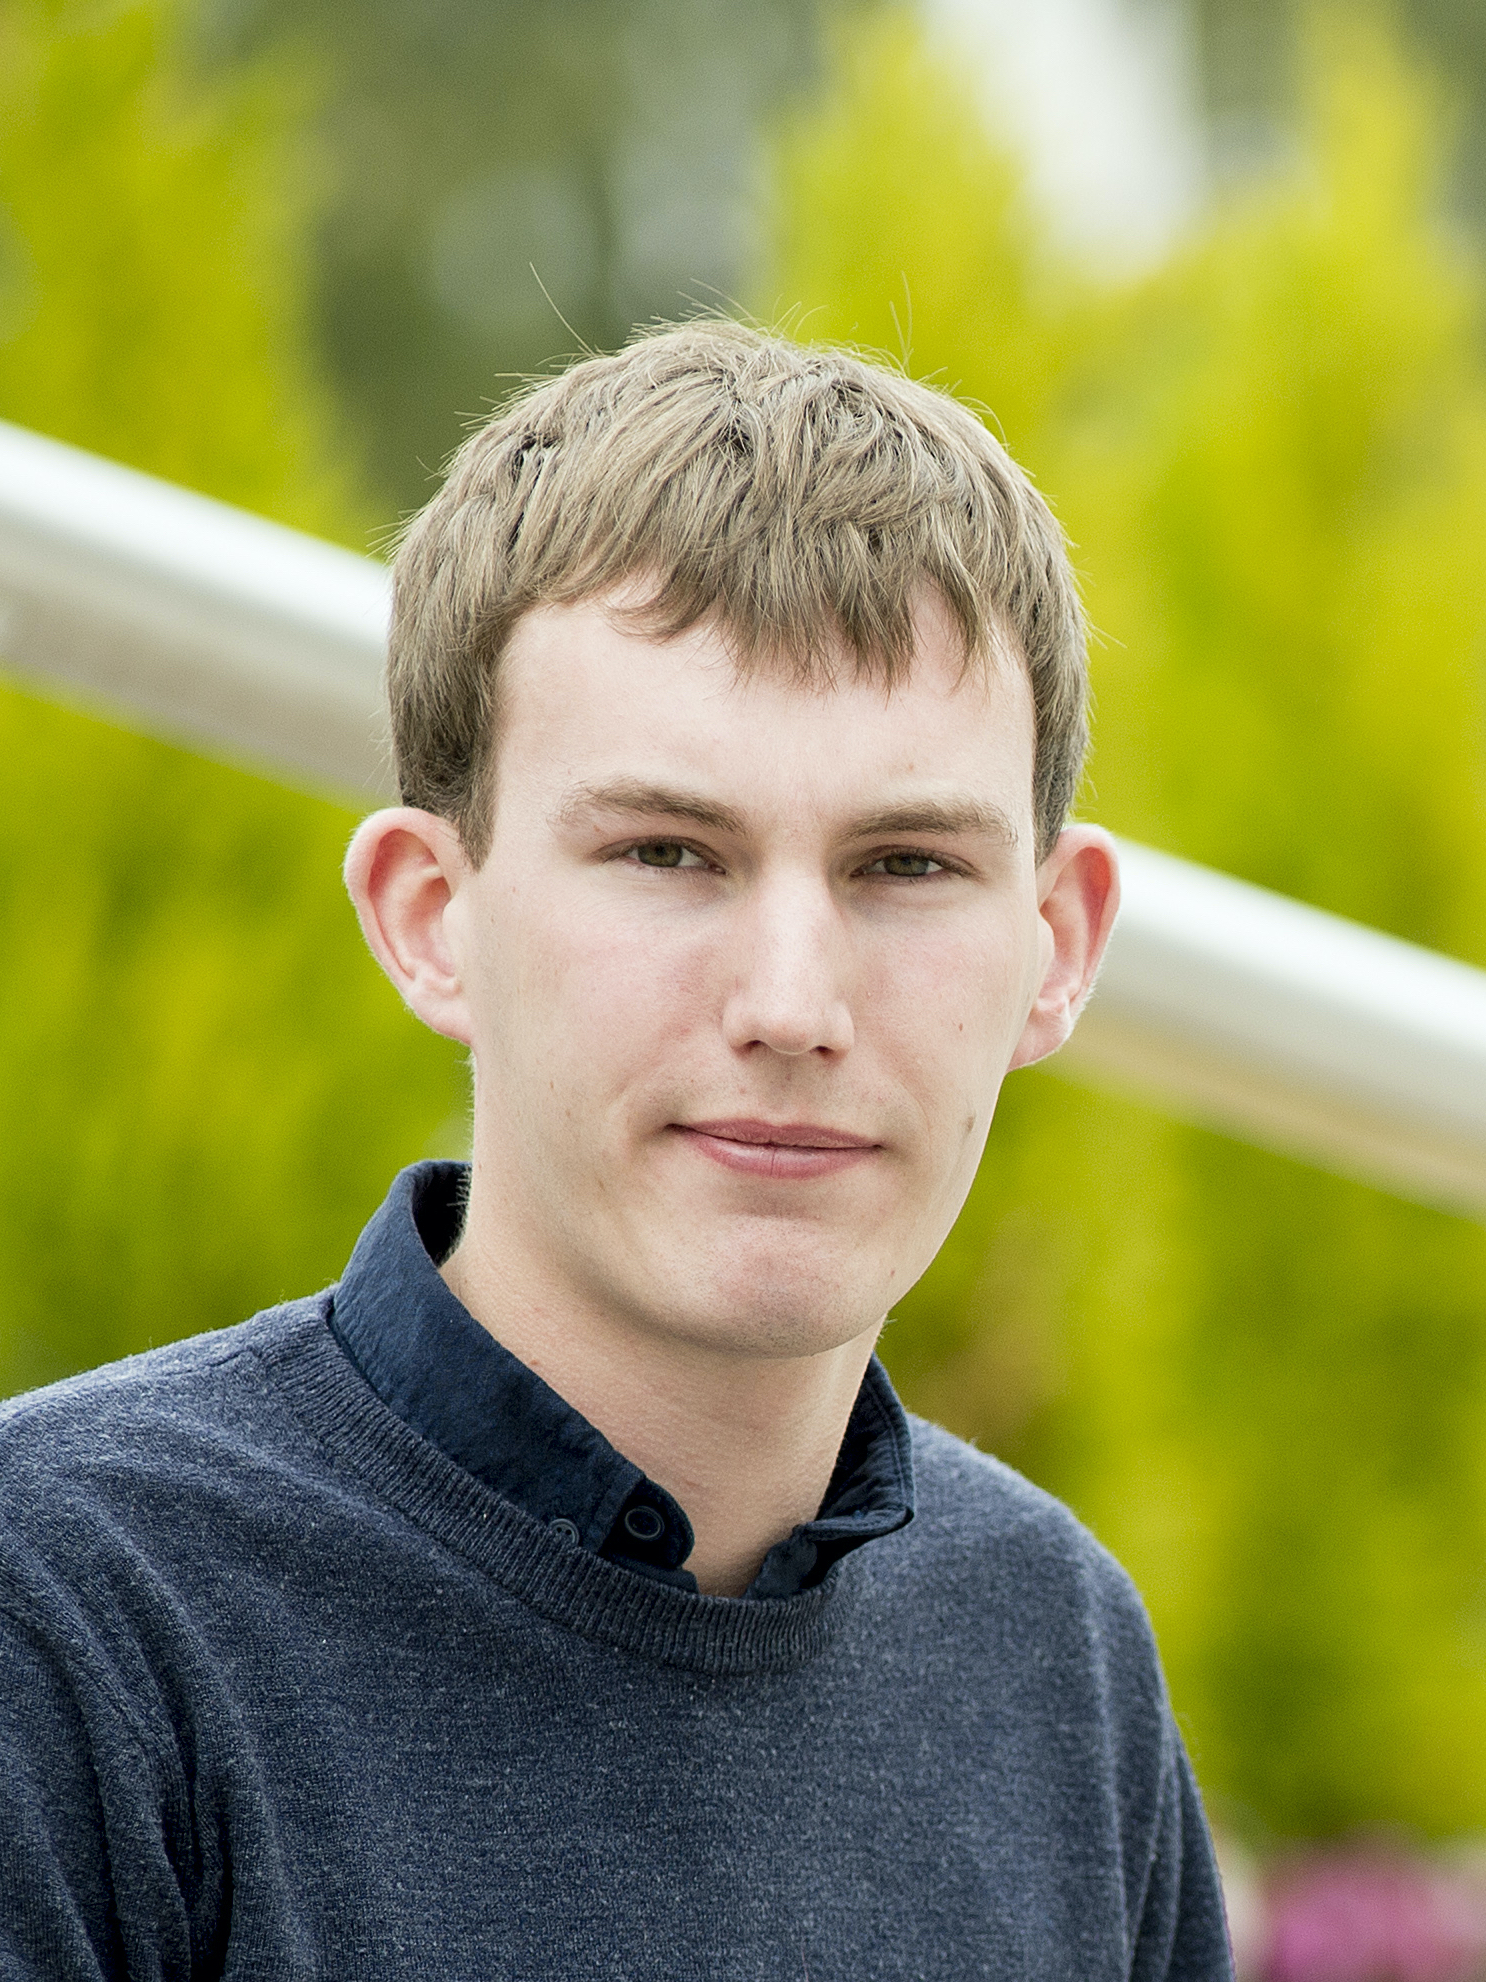
\includegraphics[width=30mm]{dp}\end{flushright}
}

\maketitlee

\href{https://lics.siglog.org/newsletters/}{Past Issues}
 - 
\href{https://lics.siglog.org/newsletters/inst.html}{How to submit an announcement}
\section{Table of Content}\begin{itemize}\item DEADLINES (\cref{deadlines}) 
 
\item SIGLOG MATTERS 
 
\begin{itemize}\item LICS 2022 (\cref{LICS2022})
\end{itemize} 
\item CALLS 
 
\begin{itemize}\item Proof Society (CALL FOR PARTICIPATION) (\cref{ProofSociety})
\item LACompLing2021 (CALL FOR PAPERS) (\cref{LACompLing2021})
\item RSSRail 2022 (CALL FOR PAPERS) (\cref{RSSRail2022})
\item NLPinAI 2022 (CALL FOR PAPERS) (\cref{NLPinAI2022})
\item CiE 2022 (CALL FOR PAPERS) (\cref{CiE2022})
\item CAV 2022 (CALL FOR PAPERS) (\cref{CAV2022})
\item FSCD 2023 (CALL FOR LOCATION) (\cref{FSCD2023})
\item ICALP 2022 (CALL FOR PAPERS) (\cref{ICALP2022})
\end{itemize} 
\item JOB ANNOUNCEMENTS 
 
\begin{itemize}\item Research Team Leader, Warsaw, Poland (\cref{ResearchTeamLeaderWarsawPoland})
\item Associate Professorship/Professorship in Automated Verification with a tutorial fellowship at Trinity College, University of Oxford (\cref{AssociateProfessorshipProfessorshipinAutomatedVerificationwithatutorialfellowshipatTrinityCollegeUniversityofOxford})
\end{itemize} 
\end{itemize}\section{Deadlines}\label{deadlines}\rowcolors{1}{white}{gray!25}\begin{tabulary}{\linewidth}{LL}Proof Society:  & Nov 08, 2021 (Workshop contributed talks abstracts), Nov 15, 2021 (Early registration closes) \\
LACompLing2021:  & Nov 14, 2021 (Paper Submission) \\
ICALP 2022:  & Nov 19, 2021 (Workshop proposal deadline), Feb 09, 2022 (Paper) \\
RSSRail 2022:  & Nov 25, 2021 (Abstract), Dec 02, 2021 (Full paper) \\
NLPinAI 2022:  & Nov 26, 2021 (Paper Submission) \\
NFM 2022:  & Dec 03, 2021 (Abstract), Dec 10, 2021 (Paper) \\
CiE 2022:  & Jan 14, 2022 (Article registration, abstract), Jan 28, 2022 (Article) \\
LICS 2022:  & Jan 17, 2022 (Titles and Short Abstracts Due), Jan 21, 2022 (Full Papers Due) \\
CAV 2022:  & Jan 21, 2022 (Paper) \\
FSCD 2022:  & Jan 22, 2022 (Call for Locations), Feb 08, 2022 (Abstract), Feb 11, 2022 (Paper) \\
AiML 2022:  & Mar 07, 2022 (Abstracts for full papers), Mar 14, 2022 (Full papers), May 23, 2022 (Short presentations) \\
\end{tabulary}
\section{LICS 2022: Thirty-Seventh Annual ACM/IEEE Symposium on LOGIC IN COMPUTER SCIENCE}\label{LICS2022}  August 2022\\ 
  Part of Federated Logic Conference 2022 (Haifa)\\ 
  \href{https://lics.siglog.org/lics22}{https://lics.siglog.org/lics22}\\ 
  \href{https://floc2022.org/}{https://floc2022.org/}\\ 
CALL FOR PAPERS 

\begin{itemize}\item  SCOPE  
 
  The LICS Symposium is an annual international forum on theoretical and practical topics in computer science that relate to logic, broadly construed. We invite submissions on topics that fit under that rubric.  
 
  Suggested, but not exclusive, topics of interest include: automata theory, automated deduction, categorical models and logics, concurrency and distributed computation, constraint programming, constructive mathematics, database theory, decision procedures, description logics, domain theory, finite model theory, formal aspects of program analysis, formal methods, foundations of computability, foundations of probabilistic, real-time and hybrid systems, games and logic, higher-order logic, knowledge representation and reasoning, lambda and combinatory calculi, linear logic, logic programming, logical aspects of AI, logical aspects of bioinformatics, logical aspects of computational complexity, logical aspects of quantum computation, logical frameworks, logics of programs, modal and temporal logics, model checking, process calculi, programming language semantics, proof theory, reasoning about security and privacy, rewriting, type systems, type theory, and verification. 
 
\item  COVID-19 etc.. 
 
  For people who cannot travel to Israel, the possibility of remote participation will be ensured. 
 
\item  IMPORTANT DATES 
 
  Authors are required to submit a paper title and a short abstract of about 100 words in advance of submitting the extended abstract of the paper. The exact deadline time on these dates is given by anywhere on earth (AoE). 
 
\rowcolors{1}{white}{gray!25}\begin{tabulary}{\linewidth}{LL}Titles and Short Abstracts Due:  & Jan 17, 2022 \\
Full Papers Due:  & Jan 21, 2022 \\
Author Feedback/Rebuttal Period:  & Mar 10-13, 2022 \\
Author Notification:  & Apr 14, 2022 \\
Conference:  & Aug 2-5,  2022 (tentative) \\
FLOC:  & Jul 31-Aug 12, 2022. \\
\end{tabulary}
 
  Submission deadlines are firm; late submissions will not be considered. All submissions will be electronic via \href{https://www.easychair.org/conferences/?conf=lics2022}{https://www.easychair.org/conferences/?conf=lics2022}. 
 
\item  SUBMISSION INSTRUCTIONS 
 
  Every full paper must be submitted in the ACM SIGPLAN Proceedings 2-column 10pt format and may be at most 12 pages, excluding references. Latex style files and further submission information is at \href{https://lics.siglog.org/lics22/cfp.php}{https://lics.siglog.org/lics22/cfp.php}.  
 
  LICS 2022 will use a lightweight double-blind reviewing process. Following this process means that reviewers will not see the authors’ names or affiliations as they initially review a paper. The authors’ names will then be revealed to the reviewers only once their reviews have been submitted. Please see the website for further details and requirements from the double-blind process. 
 
\item  LICS DISTINGUISHED PAPERS  
 
  Around 10% of accepted LICS papers will be selected as distinguished papers. These are papers that, in the view of the LICS programme committee, make exceptionally strong contribution to the field and should be read by a broad audience due their relevance, originality, significance and clarity. 
 
\item  KLEENE AWARD FOR BEST STUDENT PAPER 
 
  An award in honour of the late Stephen C. Kleene will be given for the best student paper(s), as judged by the program committee. 
 
\item  SPECIAL ISSUES 
 
  Full versions of up to three accepted papers, to be selected by the program committee, will be invited for submission to the Journal of the ACM. Additional selected papers will be invited to a special issue of Logical Methods in Computer Science. 
 
\item  PUBLICATION 
 
  The official publication date may differ from the first day of the conference. The official publication date may affect the deadline for any patent filings related to published work. We will clarify the official publication date in due course. 
 
\end{itemize}\section{Proof Society: The Proof Society Workshop on Proof Theory and its Applications and the Winter School on Proof Theory}\label{ProofSociety}  \href{https://kgs.logic.at/madeira2021/}{https://kgs.logic.at/madeira2021/}\\ 
  Madeira, Nov 29-Dec 3, 2021 \\ 
CALL FOR PARTICIPATION 

\begin{itemize}\item  We are very happy to announce the third edition of The Proof Society Workshop on Proof Theory and its Applications together with the Winter School on Proof Theory. The event will be attending-only and shall not be streamed online.  
 
  The intended audience for the Winter School is advanced master students, PhD students, postdocs and experienced researchers new to the field in mathematics, computer science and philosophy. The workshop will bring together researchers on proof theory and its applications through a series of invited and contributed talks as well as panel discussion. 
 
\item  Confirmed speakers include: 
 
\begin{itemize}\item Bahareh Afshari  
\item Juan Aguilera  
\item Eduardo Fermé  
\item David Fernández Duque  
\item Anupam Das  
\item Graham Leigh  
\item Alexander Leitsch  
\item Fedor Pakhomov  
\item Norbert Preining  
\item Michael Rathjen
\end{itemize} 
\item   IMPORTANT DATES  
 
\rowcolors{1}{white}{gray!25}\begin{tabulary}{\linewidth}{LL}Workshop contributed talks abstracts submission:  & Nov 08, 2021 \\
Early registration closes:  & Nov 15, 2021 \\
Notification:  & Nov 11, 2021 \\
Winter School on Proof Theory and its Applications:  & Nov 29—Dec 1, 2021; \\
Workshop on Proof Theory:  & Dec 2-3, 2021 \\
\end{tabulary}
 
\end{itemize}\section{LACompLing2021: Logic and Algorithms in Computational Linguistics 2021}\label{LACompLing2021}  10 - 17 December 2021, online, part of the week Mathematical Linguistics (MALIN) 2021\\ 
  \href{https://staff.math.su.se/rloukanova/LACompLing2021-web/}{https://staff.math.su.se/rloukanova/LACompLing2021-web/}\\ 
CALL FOR PAPERS 

\begin{itemize}\item  DESCRIPTION of LACompLing 
 
  Computational linguistics studies natural language in its various manifestations from a computational point of view, both on the theoretical level (modeling grammar modules dealing with natural language form and meaning, and the relation between these two) and on the practical level (developing applications for language and speech technology). Right from the start in the 1950s, there have been strong links with computer science, logic, and many areas of mathematics - one can think of Chomsky's contributions to the theory of formal languages and automata, or Lambek's logical modeling of natural language syntax. The symposium assesses the place of logic, mathematics, and computer science in present day computational linguistics. It intends to be a forum for presenting new results as well as work in progress. 
 
\item  SCOPE of LACompLing 
 
  The symposium focuses mainly on logical approaches to computational processing of natural language, and on the applicability of methods and techniques from the study of artificial languages (programming/logic) in computational linguistics. We invite participation and submissions from other relevant approaches too, especially if they can inspire new work and approaches. 
 
\item  TOPICS The topics of LACompLing2021 include, but are not limited to: 
 
\begin{itemize}\item  Computational theories of human language
\item  Computational syntax
\item  Computational semantics
\item  Computational syntax-semantics interface
\item  Interfaces between morphology, lexicon, syntax, semantics, speech, text, pragmatics
\item  Computational grammar
\item  Logic and reasoning systems for linguistics
\item  Type theories for linguistics
\item  Models of computation and algorithms for linguistics
\item  Computational approaches of computational linguistics for domain specific areas
\item  Language processing
\item  Parsing algorithms
\item  Generation of language from semantic representations
\item  Large-scale grammars of natural languages
\item  Multilingual processing
\item  Computational theories and systems of reasoning in natural language
\item  Data science in language processing
\item  Machine learning of language
\item  Interdisciplinary methods
\item  Integration of formal, computational, model theoretic, graphical, diagrammatic, statistical, and other related methods
\item  Logic for information extraction or expression in written and / or spoken language
\item  Language theories based on biological fundamentals of information and languages
\item  Computational neuroscience of language
\end{itemize} 
  LACompLing2021 is especially interested in topics on the interconnections between Logic, Language, and Argumentation, e.g.: 
 
\begin{itemize}\item  Formal languages of reasoning and argumentation
\item  Algorithms related to natural language of argumentation    
\item  theories, implementations, applications
\item  Formal models of argumentations
\item  Logic of preferences
\item  Beliefs, attitudes, persuasions - theories and applications
\end{itemize} 
\item  IMPORTANT DATES 
 
\rowcolors{1}{white}{gray!25}\begin{tabulary}{\linewidth}{LL}Paper Submission:  & Nov 14, 2021 \\
Notifications:  & Nov 21, 2021 \\
Final submissions:  & TBA \\
LACompLing2021:  & Dec 13-17, 2021 \\
\end{tabulary}
 
\item  SUBMISSION INSTRUCTIONS 
 
  We welcome submissions of abstracts of presentations of original work. The intended papers should not be submitted concurrently to another conference or conference event and should not have been published or submitted for publication consideration elsewhere. NOTE: We will not accept submissions that are on work submitted to another event at MALIN 2021, concurrently during the submission to LACompLing2021. 
 
\begin{itemize}\item  Submission of abstracts of presentations: limited to 1 page, including the title, other heading material, about half of a page text, and references
\item  Authors can submit more than one abstract. Invited speakers can submit invited and contributed abstracts. 
\item  The camera-ready submissions may require all the necessary typesetting sources, which are not in the standard LaTeX distribution
\end{itemize} 
\item  Typesetting Instructions  
 
  For LaTeX, authors are required to use Springer LNCS package, please use BibTeX style spmpsci. 
 
\item  SUBMISSIONS 
 
  \href{https://easychair.org/conferences/?conf=lacompling2021}{https://easychair.org/conferences/?conf=lacompling2021} 
 
\item  PUBLICATIONS 
 
  We will organize a post-conference, special volume after the symposium LACompLing2021, for publication of extended papers based on accepted abstracts with presentations at LACompLing2021. The submissions to the special volume have to be original, unpublished, and not concurrently submitted elsewhere. They will go through thorough peer reviews. 
 
\end{itemize}\section{RSSRail 2022: International Conference on Reliability, Safety and Security of Railway Systems}\label{RSSRail2022}  \href{https://rssrail2021.univ-gustave-eiffel.fr/}{https://rssrail2021.univ-gustave-eiffel.fr/}\\ 
CALL FOR PAPERS 

\begin{itemize}\item  The 4th International Conference on Reliability, Safety and Security of Railway Systems will be held on the 1st and 2nd of June 2022, in the International Union of Railways Congress Center, Paris. 
 
  RSSRail 2022 will address challenges currently faced by the railway industry such as: 
 
\begin{itemize}\item  improving system safety
\item  decreasing production costs and time to market
\item  reducing carbon emissions and running costs
\item  increasing the capacity of the railway.
\end{itemize} 
  Railway systems are now being integrated into larger multi-transport networks. Such systems require an even higher degree of automation at all levels of operation. These trends dramatically increase the complexity of railway applications and pose new challenges in developing novel methods of modelling, analysis, verification and validation to ensure their reliability, safety and security, as well as in supporting novel mechanisms and procedures to help make the case that development processes meet the mandated standards.  
 
\item  Development of the complex railway systems of the future requires integrated  environments and methods that support different abstraction levels and  different views, including:  
 
\begin{itemize}\item  systems architecture 
\item  safety analysis 
\item  security analysis 
\item  verification tools and methods. 
\end{itemize} 
  The conference aims to bring together researchers and engineers interested  in building critical railway applications and systems. This will be a working  conference in which research challenges and progress will be discussed and  evaluated by both researchers and engineers, focusing on their potential  to be deployed in industrial settings.  
 
\item  Topics of particular interest include:  
 
\begin{itemize}\item  safety in development processes and safety management 
\item  combined approaches to safety and security 
\item  system and software safety analysis 
\item  formal modelling and verification techniques 
\item  system reliability 
\item  validation according to the standards 
\item  safety and security argumentation 
\item  fault and intrusion modelling and analysis 
\item  evaluation of system capacity, energy consumption, cost   and their interplay 
\item  tool and model integration, toolchains 
\item  domain-specific languages and modelling frameworks 
\item  model reuse for reliability, safety and security 
\item  modelling for maintenance strategy engineering. 
\end{itemize} 
\item  Submissions 
 
\begin{itemize}\item  Research papers – not more than 16 pages in length
\item  Industrial experience reports – not more than 10 pages in length
\item  PhD student papers – not more than 10 pages in length.
\end{itemize} 
  To submit your paper please go to the conference submission site. Submissions must be formatted in the Springer LNCS format. Accepted papers will be published by Springer in a volume in the LNCS series.  
 
\item  IMPORTANT DATES 
 
\rowcolors{1}{white}{gray!25}\begin{tabulary}{\linewidth}{LL}Abstract submission:  & Nov 25, 2021 \\
Full paper submission:  & Dec 02, 2021 \\
Notification:  & Feb 01, 2022 \\
Camera-ready papers submitted:  & Mar 01, 2022 \\
\end{tabulary}
 
\end{itemize}\section{NLPinAI 2022: Natural Language Processing in Artificial Intelligence}\label{NLPinAI2022}  Online 4-6 February, 2022 \\ 
  \href{http://www.icaart.org/NLPinAI.aspx?y=2022}{http://www.icaart.org/NLPinAI.aspx?y=2022}\\ 
  Special Session within the 14th International Conference on Agents and Artificial Intelligence - ICAART 2022 \href{http://www.icaart.org}{http://www.icaart.org}\\ 
CALL FOR PAPERS 

\begin{itemize}\item  SCOPE  
 
  Computational and technological developments that incorporate natural language are proliferating. Adequate coverage encounters difficult problems related to partiality, underspecification, and context-dependency, which are signature features of information in nature and natural languages. Furthermore, agents (humans or computational systems) are information conveyors, interpreters, or participate as components of informational content. Generally, language processing depends on agents' knowledge, reasoning, perspectives, and interactions. 
 
  The session covers theoretical work, applications, approaches, and techniques for computational models of information and its presentation by language (artificial, human, or natural in other ways). The goal is to promote computational systems of intelligent natural language processing and related models of thought, mental states, reasoning, and other cognitive processes. 
 
\item  TOPICS 
 
  We invite contributions relevant to the following topics, without being limited to them: 
 
\begin{itemize}\item  Type theories for applications to language and information processing
\item  Computational grammar
\item  Computational syntax
\item  Computational semantics of natural languages
\item  Computational syntax-semantics interface
\item  Interfaces between morphology, lexicon, syntax, semantics, speech, text, pragmatics
\item  Parsing
\item  Multilingual processing
\item  Large-scale grammars of natural languages
\item  Interfaces between morphology, lexicon, syntax, semantics, speech, text, pragmatics
\item  Models of computation and algorithms for natural language processing
\item  Computational models of partiality, underspecification, and context-dependency
\item  Models of situations, contexts, and agents, for applications to language processing
\item  Information about space and time in language models and processing
\item  Models of computation and algorithms for linguistics
\item  Data science in language processing
\item  Machine learning of language
\item  Interdisciplinary methods
\item  Integration of formal, computational, model theoretic, graphical, diagrammatic, statistical, and other related methods
\item  Logic for information extraction or expression in written and spoken language
\item  Language processing based on biological fundamentals of information and languages
\item  Computational neuroscience of language
\end{itemize} 
\item  IMPORTANT DATES 
 
\rowcolors{1}{white}{gray!25}\begin{tabulary}{\linewidth}{LL}Paper Submission:  & Nov 26, 2021 \\
Authors Notification:  & Dec 14, 2021 \\
Camera Ready and Registration:  & Dec 22, 2021 \\
\end{tabulary}
 
\item  PAPER SUBMISSION  
 
  Prospective authors are invited to submit papers in any of the topics listed above. 
 
  Instructions for preparing the manuscript (in LaTeX and Word styles) are available on the ICAART pages. 
 
  Please read the Guidelines of NLPinAI 2022 at ICAART, and respect the double-blind review method: \href{http://www.icaart.org/Guidelines.aspx}{http://www.icaart.org/Guidelines.aspx} 
 
  Papers must be submitted electronically via the web-based submission system using the button SUBMIT PAPER on the pages of  NLPinAI 2022 at ICAART 2022. 
 
  All accepted papers will be published in a special section of the conference proceedings book. We expect a post-conference, post-proceedings Special Issue with extended publications based on selected papers presented at NLPinAI 2022, ICAART 2022. 
 
\end{itemize}\section{CiE 2022: Computability in Europe 2022: Revolutions and revelations in computability}\label{CiE2022}  Swansea, Wales, United Kingdom\\ 
  July 11-15, 2022\\ 
  \href{https://cs.swansea.ac.uk/cie2022/}{https://cs.swansea.ac.uk/cie2022/}\\ 
  Submission link: \href{https://easychair.org/conferences/?conf=cie2022}{https://easychair.org/conferences/?conf=cie2022}\\ 
CALL FOR PAPERS 

\begin{itemize}\item  IMPORTANT DATES (AOE): 
 
\rowcolors{1}{white}{gray!25}\begin{tabulary}{\linewidth}{LL}Article registration, abstract submission:  & Jan 14, 2022 \\
Article submission:  & Jan 28, 2022 \\
Notification of acceptance:  & Apr 11, 2022 \\
Final versions due:  & Apr 25, 2022 \\
Deadline for informal presentations submission:  & May 01, 2022 \\
Early registration before:  & May 15, 2022 \\
\end{tabulary}
 
  The notifications of acceptance for informal presentations will be sent a few days after submission. 
 
\item  CiE 2022 is the 18th conference organized by CiE (Computability in Europe), a European association of mathematicians, logicians, computer scientists, philosophers, physicists and others interested in new developments in computability and their underlying significance for the real world. 
 
\item  TUTORIAL SPEAKERS: 
 
\begin{itemize}\item  Noam Greenberg (Victoria University of Wellington)
\item  Karoliina Lehtinen (LIS, Aix-Marseille University)
\end{itemize} 
\item  INVITED SPEAKERS: 
 
\begin{itemize}\item  Erika Ábrahám (RWTH Aachen University)
\item  Thierry Coquand (University of Gothenburg)
\item  Liesbeth de Mol (Université de Lille)
\item  Damir Dzhafarov (University of Connecticut)
\item  Harvey Friedman (The Ohio State University)
\item  Svetlana Selivanova (Korea Advanced Institute of Science and Technology - KAIST)
\end{itemize} 
\item  SPECIAL SESSIONS: 
 
\begin{itemize}\item  At the intersection of computability and other areas of mathematics, organised by Denis Hirschfeldt (University of Chicago) and Karen Lange (Wellesley College)
\item  Computability theory of blockchain technology, organised by Arnold Beckmann (Swansea University) and Anton Setzer (Swansea University)
\item  Computing Language: Love Letters, Large Models and NLP, organised by Liesbeth de Mol (Université de Lille) and Giuseppe Primiero (University of Milan) for the Council of the HaPoC Commission
\item  Computing with bio-molecules, organised by Jérôme Durand-Lose (Université d'Orleans) and Claudio Zandron (University of Milan Bicocca)
\item  Constructive and reverse mathematics, organised by Samuele Maschio (Universita di Padova) and Takako Nemoto (Japan Advanced Institute of Science and Technology - JAIST)
\item  Reachability problems, organised by Paul Bell (Loughborough University) and Igor Potapov (University of Liverpool)
\end{itemize} 
\item  SUBMISSION 
 
  \href{https://easychair.org/conferences/?conf=cie2022}{https://easychair.org/conferences/?conf=cie2022} 
 
  Papers must be submitted in PDF format, using the LNCS style, max 12 pages (including references, excluding appendix)  
 
  Papers building bridges between different parts of the research community are particularly welcome. 
 
  The CONFERENCE PROCEEDINGS will be published by LNCS, Springer-Verlag. 
 
\item  INFORMAL PRESENTATIONS: 
 
  Continuing the tradition of past CiE conferences, we invite researchers to present informal presentations of their recent work. A proposal for an informal presentation must be submitted via EasyChair using the LNCS style file and be 1 page long; a brief description of the results suffices and an abstract is not required. Informal presentations will not be published in the LNCS conference proceedings. Results presented as informal presentations at CiE 2022 may appear or may have appeared in other conferences with formal proceedings and/or in journals.  
 
\item  WOMEN IN COMPUTABILITY: 
 
  We are very happy to announce that within the framework of the Women in Computability program, we are able to offer some grants for junior women researchers who want to participate in CiE 2022. Applications for this grant should be sent to Liesbeth de Mol, liesbeth.demol@univ-lille3.fr, before May 15, 2022 and include a short cv (at most 2 pages) and contact information for an academic reference. Preference will be given to junior women researchers who are presenting a paper (including informal presentations) at CiE 2022. 
 
\end{itemize}\section{CAV 2022: 34th International Conference on Computer-Aided Verification}\label{CAV2022}  August 7-10 2022, Technion, Haifa, Israel\\ 
  part of FLoC \href{https://floc2022.org/}{https://floc2022.org/}\\ 
  \href{http://i-cav.org/2022}{http://i-cav.org/2022}\\ 
  Full information at: \href{http://i-cav.org/2022/call-for-papers/}{http://i-cav.org/2022/call-for-papers/}\\ 
CALL FOR PAPERS 

\begin{itemize}\item  IMPORTANT DATES (AoE) 
 
\rowcolors{1}{white}{gray!25}\begin{tabulary}{\linewidth}{LL}Paper submission:  & Jan 21, 2022 \\
Rebuttal period:  & Mar 23-25, 2022 \\
Author notification:  & Apr 30, 2022 \\
Artifact submission:  & TBD \\
Artifact notification:  & TBD \\
Final version due:  & TBD \\
CAV AWARD Nomination deadline:  & Feb 20, 2022 \\
Main conference:  & Aug 7-10, 2022 \\
\end{tabulary}
 
\item  SCOPE  
 
  CAV 2022 is the 34th in a series dedicated to the advancement of the theory and practice of computer-aided formal analysis methods for hardware and software systems. The conference covers the spectrum from theoretical results to concrete applications, with an emphasis on practical verification tools and the algorithms and techniques that are needed for their implementation. CAV considers it vital to continue spurring advances in hardware and software verification while expanding to new domains such as machine learning, autonomous systems, and computer security. The proceedings of the conference will be published in the Springer-Verlag Lecture Notes in Computer Science series. A selection of papers is expected to be invited to a special issue of Formal Methods in System Design and the Journal of the ACM. 
 
  The conference will take place as part of Federated Logic Conference (FLoC) on August 7-10, 2022 in Technion campus, Haifa, Israel (if the pandemic and the world permit). 
 
\end{itemize}\section{FSCD 2023: Formal Structures for Computation and Deduction}\label{FSCD2023}CALL FOR LOCATION 

\begin{itemize}\item   The FSCD conference covers all aspects of Formal Structures for Computation and Deduction from theoretical foundations to applications. The annual FSCD conference comprises the main conference and a considerable number of affiliated workshops (expectedly, more than ten). 
 
  We invite proposals for locations to host the 8th FSCD International Conference to be held during the summer of 2023. Previous (and upcoming) FSCD meetings include: 
 
\begin{itemize}\item  FSCD 2016 in Porto (Portugal);
\item  FSCD 2017 in Oxford (UK) co-located with ICFP 2017;
\item  FSCD 2018 in Oxford (UK) as part of FLoC 2018;
\item  FSCD 2019 in Dortmund (Germany);
\item  FSCD 2020 in Paris (France) co-located with IJCAR 2020;
\item  FSCD 2021 in Buenos Aires (Argentina);
\item  FSCD 2022 in Haifa (Israel) as part of FLoC 2022.
\end{itemize} 
\item  The deadline for proposals is  Jan 22, 2022. Proposals should be sent to the FSCD Steering Committee Chair (see contact information below). We encourage proposers to register their intention informally as soon as possible. 
 
  The proposals will be put forward to the FSCD mailing list for an indicative vote (the results of which will not be made public), after which the final decision about hosting and organising of FSCD 2023 will be taken by the SC. 
 
\item  Proposals should address the following points: 
 
\begin{itemize}\item  FSCD Conference Chair (complete name and current position), host institution, FSCD Local Committee (complete names and current positions), availability of student-volunteers.
\item  National, regional, and local government and industry support, both organizational and financial.
\item  Accessibility to the location (i.e., transportation) and attractiveness of the proposed site. Accessibility can include both information about local transportation and travel information to the location (flight and/or train connections), as well as estimated costs.
\item  Appropriateness of the proposed dates (including consideration of holidays/other events during the period), hotel prices, and access to dormitory facilities for students.
\item  Estimated costs on registration for the conference and workshops, both for regular and student participants.
\item  Conference and exhibit facilities for the anticipated number of registrants (typically around 200). For example: number, capacity and audiovisual equipment of meeting rooms; a large plenary session room that can hold all the registrants; enough rooms for parallel sessions/workshops/tutorials; internet connectivity and workstations for demos/competitions; catering services; and presence of professional staff.
\item  Residence accommodations and food services in a range of price categories and close to the conference venue, for example, number and cost range of hotels, and availability and cost of dormitory rooms (e.g., at local universities) and kind of services they offer.
\item  Other relevant information, which can include information about leisure activities and attractiveness of the location (e.g., cultural and historical aspects, touristic activities, etc...).
\end{itemize} 
\item  Contact information: 
 
  Herman Geuvers (FSCD SC Chair): herman@cs.ru.nl 
 
\end{itemize}\section{ICALP 2022: The 49th International Colloquium on Automata, Languages, and Programming}\label{ICALP2022}   Paris, France, and online, 4-8 July 2022\\ 
   \href{https://icalp2022.irif.fr/}{https://icalp2022.irif.fr/}\\ 
CALL FOR PAPERS 

\begin{itemize}\item  The 2022 edition has the following special features: 
 
\begin{itemize}\item  Submissions are anonymous, and there is a rebuttal phase.
\item  The conference is hybrid.
\item  This will be the 50th birthday of the conference and some special events are planned.
\end{itemize} 
\item  ICALP is the main conference and annual meeting of the European Association for Theoretical Computer Science (EATCS). As usual, ICALP will be preceded by a series of workshops, which will take place on July 4. The 2022 edition will be the occasion to celebrate the 50th anniversary of both EATCS and the first ICALP, which was first held in 1972 in Rocquencourt, in the Paris area. 
 
\item  IMPORTANT DATES  (AoE) 
 
\rowcolors{1}{white}{gray!25}\begin{tabulary}{\linewidth}{LL}Paper submission:  & Feb 09, 2022 \\
Rebuttal:  & Mar 21-23, 2022 \\
Notification:  & Apr 11, 2022 \\
Camera-ready version:  & Apr 25, 2022 \\
Early registration:  & TBA \\
Conference:  & Jul 4-8, 2022 \\
\end{tabulary}
 
  Deadlines are firm; late submissions will not be considered. 
 
  \href{https://easychair.org/my/conference?conf=icalp2022}{https://easychair.org/my/conference?conf=icalp2022} 
 
\item  Invited Speakers  
 
\begin{itemize}\item  Albert Atserias, Universitat Politècnica de Catalunya
\item  Constantinos Daskalakis, MIT
\item  Leslie Ann Goldberg, Oxford University
\item  Madhu Sudan, Harvard
\item  Stéphan Thomassé, ENS Lyon
\item  Santosh Vempala, Georgia Tech
\end{itemize} 
\item  Submission Guidelines  
 
\begin{itemize}\item  Papers must present original research on the theory of computer science. No prior publication or no simultaneous submission. Authors are encouraged to also make full versions of their submissions freely accessible in an on-line repository such as ArXiv, HAL, ECCC.
\item   EasyChair, PDF, LIPIcs style, Max 15 pages (excluding references and appendix (read at the discretion of program committee members)). The extended abstract has to present the merits of the paper and its main contributions clearly, and describe the key concepts and technical ideas used to obtain the results. Submissions must provide the proofs which can enable the main mathematical claims of the paper to be fully verified.
\item  Lightweight double-blind (anonymous). See full CfP for rules.
\item   During the rebuttal phase, authors will have three days, March 21-23, to view and respond to initial reviews. Further instructions will be sent to authors of submitted papers before that time.
\item   One author per accepted paper is expected to present the work in Paris, unless there are strong reasons not to do so, including high environmental cost of travel or impossibility to travel. We will be monitoring the current situation and are aware of possible travel restrictions, but we aim to organize the conference as a hybrid event with a strong in-person attendance. If no speaker can attend, a remote presentation and participation to the discussion session are mandatory.
\item   Papers authored only by students should be marked as such upon submission in order to be eligible for the best student paper awards of the track.
\item  Accepted papers will be published in LIPIcs (open access).
\end{itemize} 
\item  AWARDS   
 
  During the conference, the following awards will be given: 
 
\begin{itemize}\item  the EATCS award (\href{https://eatcs.org/index.php/eatcs-award}{https://eatcs.org/index.php/eatcs-award}),
\item  the Gödel prize (\href{https://eatcs.org/index.php/goedel-prize}{https://eatcs.org/index.php/goedel-prize}),
\item  the Presburger award (\href{https://eatcs.org/index.php/presburger}{https://eatcs.org/index.php/presburger}),
\item  the EATCS distinguished dissertation award (\href{https://eatcs.org/index.php/dissertation-award}{https://eatcs.org/index.php/dissertation-award}),
\item  the best papers for Track A and track B,
\item  the best student papers for Track A and track B (see submission guidelines).
\end{itemize} 
\item  Topics    
 
  Papers presenting original research on all aspects of theoretical computer science are sought. Typical but not exclusive topics of interest are: 
 
  Track A: Algorithms, Complexity and Games 
 
\begin{itemize}\item  Algorithmic and Complexity Aspects of Network Economics
\item  Algorithmic Aspects of Biological and Physical Systems
\item  Algorithmic Aspects of Networks and Networking
\item  Algorithmic Aspects of Security and Privacy
\item  Algorithmic Game Theory and Mechanism Design
\item  Approximation and Online Algorithms
\item  Combinatorial Optimization
\item  Combinatorics in Computer Science
\item  Computational Complexity
\item  Computational Geometry
\item  Computational Learning Theory
\item  Cryptography
\item  Data Structures
\item  Design and Analysis of Algorithms
\item  Distributed and Mobile Computing
\item  Foundations of Machine Learning
\item  Graph Mining and Network Analysis
\item  Parallel and External Memory Computing
\item  Parameterized Complexity
\item  Quantum Computing
\item  Randomness in Computation
\item  Sublinear Time and Streaming Algorithms
\item  Theoretical Foundations of Algorithmic Fairness 
\end{itemize} 
  Track B: Automata, Logic, Semantics, and Theory of Programming 
 
\begin{itemize}\item  Algebraic and Categorical Models of Computation
\item  Automata, Logic, and Games
\item  Database Theory, Constraint Satisfaction Problems, and Finite Model Theory
\item  Formal and Logical Aspects of Learning
\item  Formal and Logical Aspects of Security and Privacy
\item  Logic in Computer Science and Theorem Proving
\item  Models of Computation: Complexity and Computability
\item  Models of Concurrent, Distributed, and Mobile Systems
\item  Models of Reactive, Hybrid, and Stochastic Systems
\item  Principles and Semantics of Programming Languages
\item  Program Analysis, Verification, and Synthesis
\item  Type Systems and Typed Calculi
\end{itemize} 
\end{itemize}\section{Research Team Leader, Warsaw, Poland}\label{ResearchTeamLeaderWarsawPoland}JOB ANNOUNCEMENT 

\begin{itemize}\item  The newly established IDEAS NCBR institute is looking for a position of research team leader  dealing with formal modeling and proving the security of cryptographic protocols used in blockchain technology. The research will be carried out in cooperation with the cryptography and blockchain laboratory headed by prof. Stefan Dziembowski at the University of Warsaw. 
 
\item  Requirements: 
 
\begin{itemize}\item  very good knowledge of at least one of the following theorem proving systems: Coq, Easycrypt, Why3, and Isabelle/HOL,
\item  PhD in computer science/mathematics or comparable professional experience,
\item  significant experience in communicating scientific results in English both orally and in writing,
\item  ability to understand scientific papers in English,
\item  experience in working in an international scientific environment.
\end{itemize} 
\item  Desirable qualifications: 
 
\begin{itemize}\item  scientific achievements in the field of automated theorem proving documented by publications,
\item  knowledge of scientific aspects of cryptography and blockchain technology.
\end{itemize} 
\item  We offer: 
 
\begin{itemize}\item  work on very interesting scientific projects with the possibility of implementing the obtained results in practice,
\item  frequent interaction with Prof. S. Dziembowski's scientific team implementing ERC (European Research Council) and NSC (National Science Centre) projects,
\item  opportunity to co-create a scientific team,
\item  form of employment: work contract,
\item  remuneration: PLN 15 000 gross,
\item  the Innovation Bonus - a share in the benefits of future commercialization of the results of a Research Project, constituting an additional remuneration in relation to the basic remuneration. The Innovation Bonus, depending on the adopted model of commercialization of the results of the Research Project, may take the form of: the right to participate in our income from their commercialization (in particular in the form of a license or disposal of intellectual property rights), or the right of acquisition of shares or stocks in a spin-out company commercializing such solutions.
\item  medical care
\item  multisport card
\item  group insurance
\item  lunch cards
\item  benefits from the Company Social Benefit Fund
\item  work tools: mobile phone, laptop
\item  relocation assistance
\end{itemize} 
\item  The complete set of required documents should be sent by e-mail to: jobs@ideas-ncbr.pl 
 
\end{itemize}\section{Associate Professorship/Professorship in Automated Verification with a tutorial fellowship at Trinity College, University of Oxford}\label{AssociateProfessorshipProfessorshipinAutomatedVerificationwithatutorialfellowshipatTrinityCollegeUniversityofOxford}  \href{http://www.cs.ox.ac.uk/news/1976-full.html}{http://www.cs.ox.ac.uk/news/1976-full.html}\\ 
JOB ANNOUNCEMENT 

\begin{itemize}\item  Applications are invited for the post of Associate Professor (or Professor) of Automated Verification in the Department of Computer Science and Trinity College, to start before October 2022. The successful candidate will also be appointed as a Fellow and Tutor in Computer Science at Trinity College, and will be responsible for the organisation and teaching of their subject within the College. 
 
\begin{itemize}\item  You will be a member of both the University and the College community, part of a lively and intellectually stimulating research community with access to the excellent research facilities which Oxford offers. You will have a role to play in the running of the College as a member of the Governing Body and a trustee of the College as a charity. 
\item  The Department of Computer Science is a vibrant and growing academic department, which has a research profile across the entire spectrum of contemporary computer science.  You will be expected to engage in independent and original research aligned with the Automated Verification research theme, to secure funding and engage in the management of research projects and disseminate research of the highest international standard through publications, conferences and seminars.  You will also contribute to teaching on the Department’s highly successful undergraduate and graduate programmes.
\item  You will hold a doctoral degree in Computer Science (or cognate discipline), have the ability to teach across a range of Computer Science subjects, and will also have a proven research record of high quality at international level, and experience of research collaborations at both national and international level.
\end{itemize} 
\item  APPLICATION DEADLINE AND INTERVIEW DATE  
 
\begin{itemize}\item  The closing date for applications is 12 noon on 21 January 2022.
\item  Interviews are expected to be held on 4 March 2022.
\end{itemize} 
\item  HOW TO APPLY, FURTHER PARTICULARS AND SELECTION CRITERIA 
 
\begin{itemize}\item  \href{http://www.cs.ox.ac.uk/news/1976-full.html}{http://www.cs.ox.ac.uk/news/1976-full.html}
\item  \href{http://www.cs.ox.ac.uk/files/12971/153743%20-%20Job%20Description%20and%20Selection%20Criteria.pdf}{http://www.cs.ox.ac.uk/files/12971/153743%20-%20Job%20Description%20and%20Selection%20Criteria.pdf}
\end{itemize} 
\end{itemize}


To the \href{http://siglog.org/}{SIGLOG} or \href{https://lics.siglog.org}{LICS} website\end{document}